% `template.tex', a bare-bones example employing the AIAA class.
%
% For a more advanced example that makes use of several third-party
% LaTeX packages, see `advanced_example.tex', but please read the
% Known Problems section of the users manual first.
%
% Typical processing for PostScript (PS) output:
%
%  latex template
%  latex template   (repeat as needed to resolve references)
%
%  xdvi template    (onscreen draft display)
%  dvips template   (postscript)
%  gv template.ps   (onscreen display)
%  lpr template.ps  (hardcopy)
%
% With the above, only Encapsulated PostScript (EPS) images can be used.
%
% Typical processing for Portable Document Format (PDF) output:
%
%  pdflatex template
%  pdflatex template      (repeat as needed to resolve references)
%
%  acroread template.pdf  (onscreen display)
%
% If you have EPS figures, you will need to use the epstopdf script
% to convert them to PDF because PDF is a limmited subset of EPS.
% pdflatex accepts a variety of other image formats such as JPG, TIF,
% PNG, and so forth -- check the documentation for your version.
%
% If you do *not* specify suffixes when using the graphicx package's
% \includegraphics command, latex and pdflatex will automatically select
% the appropriate figure format from those available.  This allows you
% to produce PS and PDF output from the same LaTeX source file.
%
% To generate a large format (e.g., 11"x17") PostScript copy for editing
% purposes, use
%
%  dvips -x 1467 -O -0.65in,0.85in -t tabloid template
%
% For further details and support, read the Users Manual, aiaa.pdf.


% Try to reduce the number of latex support calls from people who
% don't read the included documentation.
%
\typeout{}\typeout{If latex fails to find aiaa-tc, read the README file!}
%


\documentclass[]{aiaa-tc}% insert '[draft]' option to show overfull boxes

\usepackage{lettrine}%  dropped capital letter at beginning of paragraph
\usepackage{subfigure}% subcaptions for subfigures
\usepackage{subfigmat}% matrices of similar subfigures, aka small mulitples
\usepackage{placeins}%  figure section constraint
\usepackage{mathtools}% not sure why this is here...probs for math stuff
\usepackage{graphicx}
\graphicspath{./}
\usepackage{listings}

 \title{Final Project: \\ Blasius Boundary Layer and Poisson's Equation}

 \author{
  Ryan J. Krattiger%
    \thanks{Undergraduate Senior, Department of Mechanical and Aerospace Engineering.} \\
  {\normalsize\itshape
  Missouri University of Science and Technology, Rolla, MO, 65401, USA}
 }

 % Data used by 'handcarry' option if invoked
 \AIAApapernumber{YEAR-NUMBER}
 \AIAAconference{Conference Name, Date, and Location}
 \AIAAcopyright{\AIAAcopyrightD{YEAR}}

 % Define commands to assure consistent treatment throughout document
 \newcommand{\eqnref}[1]{(\ref{#1})}
 \newcommand{\class}[1]{\texttt{#1}}
 \newcommand{\package}[1]{\texttt{#1}}
 \newcommand{\file}[1]{\texttt{#1}}
 \newcommand{\BibTeX}{\textsc{Bib}\TeX}

\begin{document}

\maketitle

\begin{abstract}
The Blasius Boundary Layer equation and Poisson's equation were solved
in this report. The Blasius was solved for the general form; however, the solution
was not expanded on beyond the similarity solution. Poisson's equation was similarly
solved, but for a set of solvable boundary conditions. The reason for this was to
allow for a comparison of methods via error, which requires an exact solution.
It should be clear from the examples provided that the functionality developed in
these solvers is robust enough to apply the corresponding methods to a wide variety
of scientific and engineering problems.
\end{abstract}

\newpage

\tableofcontents

\lstlistoflistings

\newpage

\section*{Nomenclature}

\begin{tabbing}
  XXX \= \kill% this line sets tab stop
  $f$ \> Function \\
  $\bar x$ \> Variable value vector \\
  $\nu$ \> Dynamic viscosity \\
  $U$ \> Velocity magnitude \\
  h \> Step size \\
  x \> x-position \\
  $\delta$ \> Boundary Layer thickness \\
  $\bar r$ \> residual vector \\
  \textit{Subscript} \\
  $i$ \> Row index \\
  $j$ \> Column index \\
  $e$ \> Boundary layer edge \\
 \end{tabbing}


% ---------------------------------------------------------------------------- %
%                                 INTRODUCTION                                 %
% ---------------------------------------------------------------------------- %
\FloatBarrier\section{Introduction}
\lettrine[nindent=0pt]{F}{or} the final project it was perscribed to apply a minimum of six numerical methods
from six unique topics covered in the Applied Computational Methods course. The
problems choosen were to be from either relevent research or applications to engineering.
The two problems choosen and presented in this report include a solution to the Blasius
Boundary Layer equation and solution methods for Poisson's equation
(commonly used in eletromagnitism, 2D Heat transfer, Subsonic flow fields, etc.). The
Blasius equation used solved using the Runge-Kutta 4-step method coupled with the
secant method to provide a smart `shooting` method. Once this equation was solved,
numerical integration was carried out to verify the solution. The Poisson equation was
solved by first discretizing using central difference differentiation for a second
derivative, then assembled into a system of linear equations and sovled using the
Liebmann (Gauss-Seidel) Method and Steepest Decent Method.


% ---------------------------------------------------------------------------- %
%                                     MODEL                                    %
% ---------------------------------------------------------------------------- %
\FloatBarrier\section{Models}
This section will highlight the models used in the final project and the respective
solution methods implemented. The focus of this section is two parts. This first
is to demonstrate the physical significance of the problem and the second is to
show the general idea of what methods were implemented and why they were choosen.

% ----------------------- %
% -- Blasius BL Section --%
% ----------------------- %
\FloatBarrier\subsection{Blasius Boundary Layer}
The Blasiun equation is used to model boundary layer over a 2D flat plate as a
similarity solution. The general form of this equation is given as Eq~\ref{e:blas_diff}
where f is a function of $\eta$, the similarity parameter.

\begin{equation}
  \label{e:blas_diff}
  2 f''' + f f'' = 0
\end{equation}

In order to do this accomplish this solution Blasius first converted (x,y) pairs
to ($\xi$, $\eta$) using Eq~\ref{e:blas_trans}.

\begin{equation}
  \label{e:blas_trans}
  \xi = x \quad \textrm{and} \quad \eta = y \sqrt{\frac{U}{\nu x}}
\end{equation}

Using $\eta$ it is then possible to define the function f($\eta$) such that the stream
function ($\psi$) can be expressed as Eq~\ref{e:blas_stream}.

\begin{equation}
  \label{e:blas_stream}
  \psi = \sqrt{\nu U x} f(\eta)
\end{equation}

From the stream function the x- and y-velocity components are then easily found
by simply differentiating the stream function to obtain the results in Eq~\ref{e:blas_u}
and Eq~\ref{e:blas_v} respectively.

\begin{equation}
  \label{e:blas_u}
  u(x,\eta) = \frac{\partial \psi}{\partial y} = U f'
\end{equation}

\begin{equation}
  \label{e:blas_v}
  v(x,\eta) = -\frac{\partial \psi}{\partial x} = \sqrt{\frac{\nu U}{x}} (\eta f' - f)
\end{equation}

And further the shear stress at the wall, $\tau_{wall}$, can be found using the
gradient of the x-velocity with respect to $\eta$ as seen in Eq~\ref{e:blas_shear}.

\begin{equation}
  \label{e:blas_shear}
  \tau_{wall}(x) = \mu \frac{d u}{d \eta} \vert_{\eta=0} = \mu U f''\vert_{\eta=0}
\end{equation}

where $\mu$ is the dynamic viscosity. \\

Since it is clear that this ODE can be useful, it is now worth while to solve it.
In order to solve this ODE using a Runge-Kutta 4-step scheme it is required to
decompose the Eq~\ref{e:blas_diff} into a system of coupled first order ODEs.
This decomposition can be seen in Eq.~\ref{e:blas_cupode}.

where

\begin{equation}
\label{e:blas_cupode}
  \bar Z = \begin{bmatrix}
    z_1 \\ z_2 \\ z_3
  \end{bmatrix} =
  \begin{bmatrix}
    f \\ f' \\ f''
  \end{bmatrix}
  \quad \textrm{and} \quad
  \bar Z' = \begin{bmatrix}
    z_1' \\ z_2' \\ z_3'
  \end{bmatrix} =
  \begin{bmatrix}
    f' \\ f'' \\ f'''
  \end{bmatrix} =
  \begin{bmatrix}
    z_2 \\ z_3 \\ - \frac{1}{2} z_1 z_2
  \end{bmatrix}
\end{equation}

Additionally the boundary conditions must be provided for the initial value problem
that is to be solved. In this case it is known that the horizontal velocity (u), and so the stream
function ($\psi$) must both be zero at the wall (y=0). Additionally, it is known that
at the boundary layer edge, the velocity is equivelant to the freestream ($u=u_e$).
This translates to the boundary conditions in Eq~\ref{e:blas_bc}

\begin{equation}
  \label{e:blas_bc}
  f(0) = 0 \quad f'(0) = 0 \quad f'(\infty) = 1
\end{equation}

It is noticed that there is no initial condition for the $z_3$ or f'' term. In
to determine this value, it is required to perform the shooting method, or in
layman's terms guess. The criteria that will be met to
determine if the initial guess is good is to find where $f'(\eta_n) - 1 = 0$.
But to do a little better than just guessing, the secant method
will be used to find the zero of this criteria.

Solving $\bar Z'$ in order to determine what the values of f, $f'$, and $f''$ are
will be done using the Runge-Kutta 4-step (RK4) method dicussed in class. A note here
that any method for solving an ODE could be used here but the RK4 was choosen for
nostalgic reasons.

In the attached code the method of how the RK4 method was nested in the secant
method can be seen. The essence of the idea was to wrap the RK4 solving the given
ODE in a function of a single variable, $f''(0)$ or $z_{2,0}$, and return the result of $f'(\eta_{max}) - 1 = 0$.
Then this was nested inside of another loop that check for convergence of $f''(0)$
as $\eta_{max}$ increased in the domain $\eta_{max} \in [1,\infty)$ with increment
steps of 1. This was done to capture the effect of $\infty$ while performing the
minimum number of iterations. Note, as $\eta_{max}$ increased the step size if the
ODE solver remained at 0.1 using a scaling factor of 10 in order to maintain uniformity
in each iteration.

The last test performed for this problem was with numerical integration. In order
to verify that the f'' and f' values agree, as they should from how the problem was
defined, f'' was integrated over the interval using simpson's 1/3 rule. The reason
this method was choosen over the trapezoidal method or a gauss quadrature method
was due to the higly contoured shape of the f'' solution and the lack of an actual
function to evaluate at specific points respectively. 

% ----------------------- %
% -- Poisson's Equation --%
% ----------------------- %
\FloatBarrier\subsection{Poisson's Equation}

The poisson eqaution is used in many diciplines as it is a common mathematical
model found in physical systems. Because of the relative complexity of these
physical systems, a simplified and solvable example was used simple to demonstrate
the application of two different solution methods.

The first thing to consider is the general form of Poisson's equation as seen in
Eq~\ref{e:p_diff}. It is clear that this is a second order, linear, partial differential
equation in three dimensions, x, y. The forcing function, f(x,y), can be anything
depending on the problem and is one of five drivers for the solution.

\begin{equation}
  \label{e:p_diff}
  \frac{\partial ^2 u}{\partial x^2} + \frac{\partial ^2 u}{\partial y^2} = f(x,y)
\end{equation}

Being a second order PDE, it is required to have two boundary conditions for each
independent variable. In this case that would be x and y, resulting in a required
four boundary conditions.

For the problem to be solved here, the forcing function can be seen in Eq~\ref{e:p_f}
and the boundary conditions are writen in Eq~\ref{e:p_bcx} and q~\ref{e:p_bcy}.

\begin{equation}
  \label{e:p_f}
  f(x,y) = -2(x^2 + y^2)\quad \textrm{for} \quad (0 \leq x \leq 1, 0 \leq y \leq 1)
\end{equation}

\begin{equation}
  \label{e:p_bcx}
  u(x,0) = 1 - x^2 \quad \textrm{,} \quad u(x,1) = 2(1 - x^2) \quad \textrm{for} \quad 0 \leq x \leq 1
\end{equation}

\begin{equation}
  \label{e:p_bcy}
  u(0,y) = 1 + y^2 \quad \textrm{,} \quad u(1,y) = 0 \quad \textrm{for} \quad 0 \leq y \leq 1
\end{equation}

It can be shown that the exact solution for these constraints is as seen in Eq~\ref{e:p_exact}.

\begin{equation}
  \label{e:p_exact}
  u(x,y) = (1 - x^2)(1 + y^2)
\end{equation}

Reguardless of the forcing function and boundary conditions, the set up of the
problem is done so generically, independant of any set of inputs.

This first step is to descretize the original PDE as seen in Eq~\ref{e:p_diff} into
the form seen in Eq~\ref{e:p_num}. It can be seen that the second order, central
difference scheme was used.
\\\\
Let $u(x_i,y_j) = u_{i,j}$, where $i \in [0,N]$, $j \in [0,M]$, and $h = \frac{x_N - x_0}{N}$ and $k = \frac{y_M - y_0}{M}$

\begin{equation}
  \label{e:p_num}
  \frac{u_{i-1,j} - 2u_{i,j} + u_{i+1,j}}{h^2} + \frac{u_{i,j-1} - 2u_{i,j} + u_{i,j+1}}{k^2} = f(x_i,y_j)
\end{equation}

Further simplifying this equation and letting $\frac{h^2}{k^2} = \lambda$ gives a
general simplified form for the numerical scheme (Eq~\ref{e:p_num_simp}).

\begin{equation}
  \label{e:p_num_simp}
  - 2(\lambda + 1)u_{i,j} + \lambda u_{i-1,j} + \lambda u_{i+1,j}  + u_{i,j-1} + u_{i,j+1} = f(x_i,y_j)
\end{equation}

After some carefull consideration it can be shown that the above eqation can be
applied to the grid structure in figure~\ref{f:cdiff_grid}. It can also be seen
that at the boundaries, where the values are known from boundary conditions, can
be looked at as constants.

\begin{figure}
  \centering
  \label{f:cdiff_grid}
  \caption{Grid with points used in central difference discretized Poisson}
  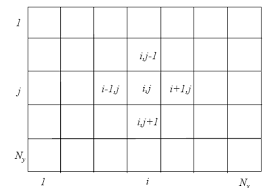
\includegraphics[width=0.5\textwidth]{cdiff_grid.png}
\end{figure}

In order to put the now discretized equation into a solvable form it is translated
to a system of linear equations. After some work a matrix-vector pair can
be found and the system and be written in the form of $A \bar x = \bar b$
\\\\
where A is an MxM block diagonal matrix
$$
\begin{bmatrix}
  T      & I     &     0   & \dots & 0 \\
  I     & T      & I     &  & \vdots \\
  0 &  & \ddots &  & 0 \\
  \vdots &   & I     & T & I \\
  0      & \dots  &  0     & I & T
\end{bmatrix}
$$
\\\\
and T is a NxN tridiagonal matrix
$$
\begin{bmatrix}
  -2(\lambda + 1)      & \lambda     &     0   & \dots & 0 \\
  \lambda     & -2(\lambda + 1)      & \lambda     &  & \vdots \\
  0 &  & \ddots &  & 0 \\
  \vdots &   & \lambda     & -2(\lambda + 1) & \lambda \\
  0      & \dots  &  0     & \lambda & -2(\lambda + 1)
\end{bmatrix}
$$
\\\\
and I is an NxN identity matrix.

In total, A is (NxM)x(NxM) which is quite large. Luckily, there is sparse matrix
support in most linear algebra/numerical libraries used in computing to handle this.

The $\bar b$ vector is composed of two parts. This first is made up of the boundary
conditions ($\bar c$), and the second is the forcing vector ($\bar d$). The resulting
$\bar b$ is the denoted as $\bar b = \bar c  + \bar d$.
\\\\
$\bar c$ can be defined as

$$
\begin{bmatrix}
  -( u_{1,0} + \lambda u_{0,1}) \\
  -u_{2,0} \\
    \vdots \\
  -( u_{N-1,0} + \lambda u_{N,1}) \\
  \lambda u_{0,2} \\
    0 \\
  \vdots \\
    0 \\
  \lambda u_{N,2} \\
  \vdots \\
  -( u_{1,M} + \lambda u_{0,M-1}) \\
  -u_{2,M-1} \\
    \vdots \\
  -( u_{N-1,M} + \lambda u_{N,M-1}) \\
\end{bmatrix}
$$
\\\\
$\bar d$ can be defined as

$$
\begin{bmatrix}
  f(x_1,y_1) \\
  f(x_1,y_2) \\
  \vdots \\
  f(x_{N-1},y_{M-1})
\end{bmatrix}
$$
\\\\
And finally $\bar x$, the solution vector is the set of unknown nodes on the grid.
The (i,j) coordinate of the grid is translated using a linear relation to give
a vectorized form of the matrix such that

$$
\begin{bmatrix}
  u_{1,1} \\
  u_{1,2} \\
  u_{1,3} \\
  \vdots \\
  u_{N-1,M-1}
\end{bmatrix}
$$

In the final form of $A \bar x = (\bar c + \bar d)$ the Poisson equation is in a
form that is solvable. The two methods that will be shown here are the Liebmann
Method (also known as the Gauss-Seidel Method) and with a Steepest Decent optimization
scheme.

\subsubsection{Liebmann Method}
As an iterative solving technique, Liebmann Method, also known as the Gauss-Seidel method,
is best applied to sparse structured matrices rather than dense matrices. The reason
for this is due to the need to perform O(N$^{2}$) operations, or one operation for
each non zero element of the matrix, to compute the values of $\bar x$ in each iteration.
If there are many non-zero values, there are more operations required for each iteration.
Since the matrix proposed above is indeed sparse, this method is more desirable than a
traditional Gauss-Eliminiation technique. Selecting an initial guess, say the $\bar b$
vector from above, it is possible to now begin iterations.

For iteration k+1, the general form for the x$_i$ element is Eq~\ref{e:lieb_it} for $i\in 0...N$
and N is the size of the solution vector.

\begin{equation}
  \label{e:lieb_it}
  x_i^{k+1} = \frac {b_i - \sum_{j=0}^{i-1} x_j^{k+1} a_{i,j} - \sum_{j=i+1}^{N} x_j^k a_{i,j}}{a_{i,i}}
\end{equation}

In implementation the solution vector would be a single variable, so as $x_i$ was
updated, the update would be seen when solving for $x_{i+1}$. With this in mind,
the above Eq~\ref{e:lieb_it} can be changed into a simpler form seen in Eq~\ref{e:lieb_it2},
recalling that the projection of two vectors (or the dot product) is
$\bar a \cdotp \bar b = \sum_{i=0}^{N} a_i b_i$. Also let $\bar a_i$ be the vector
created by the i$^{th}$ row of the matrix A.

\begin{equation}
  \label{e:lieb_it2}
  x_i = \frac {b_i - \bar a_{i} \cdotp \bar x + a_{i,i} x_i}{a_{i,i}}
\end{equation}

By iterating of Eq~\ref{e:lieb_it2} until convergence of the residual vector
$\vert\vert r_k \vert\vert_2 \leq tolerance$.
The reason to rewrite the solver in this way is to give way to allow the underlying
operation of the dot product be optimized for sparse vector types. In this sense, for
each product of the A matrix row and the current solution vector, a minimum number
of operations will be performed. This also allows for the solver to work for multiple
types of matrix problems and still obtain optimal performance without having to
write a special solver for every sparse or dense matirx used. The same idea will
be used again in the the next solver.

\subsubsection{Steepest Decent}
Another iterative solver can be used, however the Steepest Decent method looks
at this problem as an optimization problem rather than a system of linear equations
solving problem.

In general an optimization problem for a function F($\bar x$) is as follows:
\\\\
Determine a search direction $\bar s_k$
\\\\
Solve for the optimal $\alpha_k^{*}$ to find to minimum in the search direction
use the knowns $\bar x_k$ and the search direction $\bar s_k$ and then use 1D minimization
on F($x_{k+!}$($\alpha_k^{*}$)). The below is an example of using the derivative
of F to find the minimum.

$$
   F'(\bar x_{k+1}) = 0 \quad \textrm{where} \quad \bar x_{k+1} = \bar x_{k} + \alpha_k^{*} \bar s_k
$$


Finally update $\bar x$
$$
   \bar x_{k+1} = \bar x_{k} + \alpha_k^{*} \bar s_k
$$

and check if the solution meets convergence criteria using the norm of the
residual vector ($\bar r_k = A \bar x_k - \bar b$).
$$
\vert\vert r_k \vert\vert_2 \leq tolerance
$$

The current problem to be solved is $Ax-b=\bar 0$; however, a linear system is not a form that
is particularly well suited for optimization since the zero vector is not the
minimum. By integrating the system the resulting equation is $\frac{1}{2} x^T A x - x^T b = 0$.
This form of the equation does have a minimum as it is a quadratic system of eqations.
\\\\
For the Steepest Decent method, the search direction is determined by the local
direction of steepest decent, or the negative gradient. The formula for this should look
familiar as Eq~\ref{e:p_sk}, which is the residual vector.

\begin{equation}
  \label{e:p_sk}
  \bar s_k = \bar r_k = \bar b - A \bar x_k
\end{equation}

The $\alpha_k$ can be found from the above method finding the root of the derivative
as

$$
  \alpha_k = \frac{s_k \cdotp s_k}{s_k \cdotp \bar q_k}
$$

where $\bar q_k = A s_k$.
\\\\
With the search direction ($s_k$) and optimal $\alpha_k^*$ it is a simple matter
to update the solution vector. Again, this will iterator until convergence is
found.

There are two additional methods that are linked to Steepest decent. The first is
Conjugant Gradient (CGM) and the second is Preconditioned Conjugant Gradient (PCGM).
These methods both provide much faster convergence on average, but require more computations
per step. More informatoin about these, and a brief study on how they improve the
gradient based methods as applied to the solution of 2D Poisson's equation
can be found in Holmes et. al.\cite{holmes:07bk}

% ---------------------------------------------------------------------------- %
%                                   RESULTS                                    %
% ---------------------------------------------------------------------------- %
\FloatBarrier\section{Results}
The results presented here are simply to show the results and relevent error or
convergence of methods used. 

\FloatBarrier\subsection{Blasius Boundary Layer}
In figure~\ref{f:blas_plots} the solution to the $\bar Z$ parameters are shown. 
The values plotted are labeled as stream function, u/u$_e$ and shear stress but are
actually f, f', and f'' respectively. The purpose of the naming was simply to 
demonstrate the general profile of the flow for the relevent parameters calculated 
using f, f', and f''.


\begin{figure}[htb]% order of placement preference: here, top, bottom
  \caption{Results from solving the Blasius Boundary Layer equation}
  \begin{subfigmatrix}{2}
    \subfigure[Stream Function]{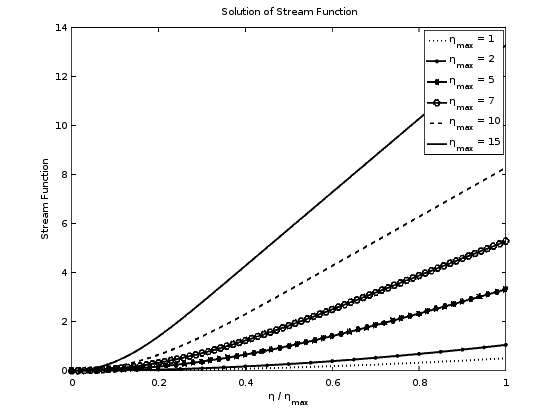
\includegraphics{stream_fnct.png}}
    \subfigure[Scaled Velocity Profile]{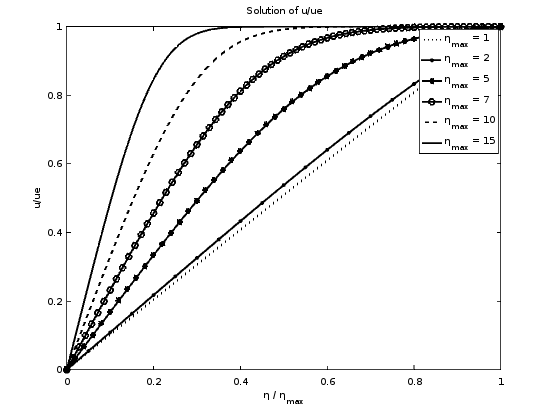
\includegraphics{uue_fnct.png}}
    \subfigure[Wall Shear Stress]{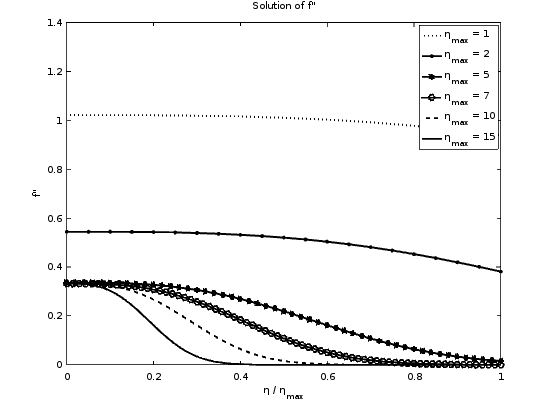
\includegraphics{fpp_fnct.png}}
  \end{subfigmatrix}
 \label{f:blas_plots}
\end{figure}

A second check to verify the solution obtained, the f'' result was integrated over
the range in the converged iteration, $\eta_{max} = 15$.

$$
  \int_{0}{15} f''(\eta) d\eta = f'(15) - f'(0) = 1
$$

The result of this integration can be seen in the table table~\ref{t:blas_interror}.
It can be seen that the numeric integral solution and the expected soltion are very close,
especially for the integration results coming as the result of two seperate numerical methods.

\begin{table}
\centering
\label{t:blas_interror}
  \begin{tabular}{l | l}
  Solution & Error \\
  \hline
  1.000023279653586 & 2.327965358617234e-05 \\
  \end{tabular}
\end{table}

\FloatBarrier\subsection{Poisson's Equation}

The figures~\ref{f:p_results} show the solution plots of each respective method.
The plot of the norm of the residual as a function of iteration for each method
is presented in figure~\ref{f:p_convergeplot}. It can be seen that the steepest decent
has a much slower convergence rate compared to the Liebmann method, taking roughly
twice as many iterations to converge. The results from comparing the solution method
for a 20x20 and 30x30 grid are not included here, but similar conclusions can be drawn. 

\begin{figure}[htb]% order of placement preference: here, top, bottom
  \caption{Results from solving the Blasius Boundary Layer equation}
  \begin{subfigmatrix}{2}
    \subfigure[Exact Solution]{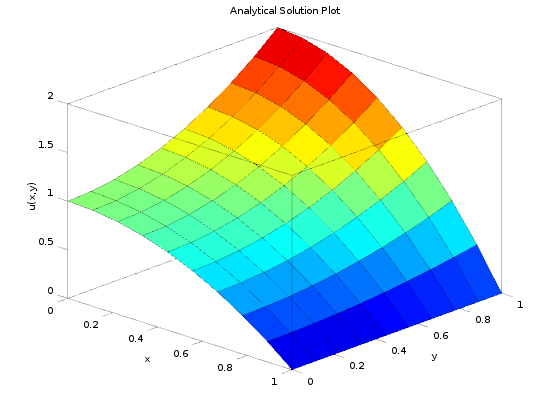
\includegraphics{pois_ana}}
    \subfigure[Steepest Decent Solution]{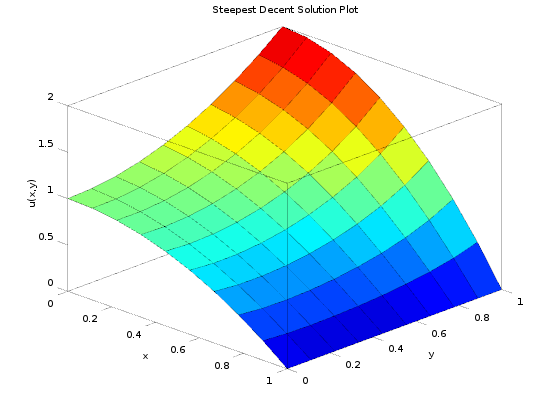
\includegraphics{pois_sd}}
    \subfigure[Liebmann Solution]{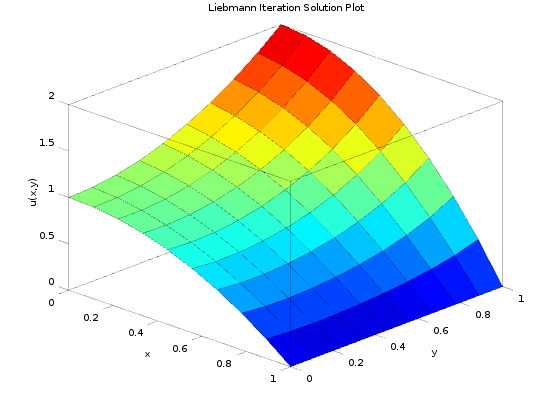
\includegraphics{pois_lieb}}
  \end{subfigmatrix}
 \label{f:p_results}
\end{figure}

\begin{figure}[htb]% order of placement preference: here, top, bottom
  \caption{Results from solving the Blasius Boundary Layer equation}
  \begin{subfigmatrix}{2}
    \subfigure[Steepest Decent error vs iteration]{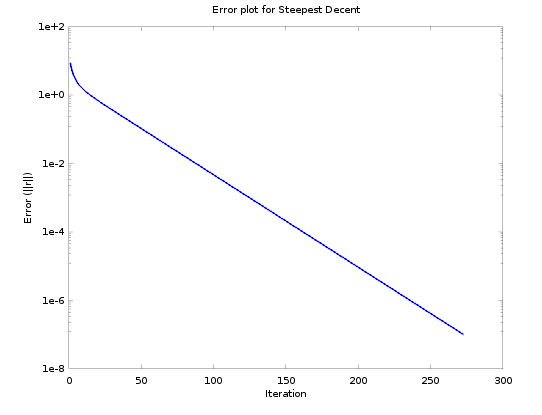
\includegraphics{sd_err}}
    \subfigure[Liebmann error vs iteration]{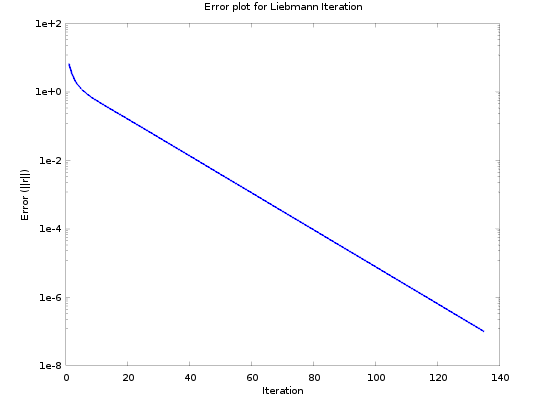
\includegraphics{lieb_err}}
  \end{subfigmatrix}
 \label{f:p_convergeplot}
\end{figure}

Notice that for both methods the number of iterations required is greater than
N. It may be tempting to say that this makes the cost of each of these methods
roughly equal to that of a Gauss-Elimination as each step appears to be around
O(N$^2$); however, that would be incorrect. Because of the sparse nature of the 
matrix a good numerical library will leverage the fact that most values are zero
and only perform operations on the non-zero values in the matrix and vector. In 
Matlab, this may not always be the case. In the numerical library
that was suppose to be used to solve this problem, and will be shortly after this
paper is submitted, the described advantages are leveraged. So the actual complexity
is only O(N) operations rather than O(N$^2$), which puts both of these methods
ahead with a total complexity of roughly O(N$^2$).

\FloatBarrier\section{Conclusion}

It is clear that the numerical methods presented, when applied correctly as
they have been here, are capable of providing extraordinarly powerful tools that
allow humans to use computers to solve ever more complicated problems that occur
in science and engineering. The study and advancement of numerical methods to solve these
problems and make more robust and smarted (adaptive) solvers has been the key to increasing design and
analysis speed in the past and will continue to be so in the future. Not to be
excited about computing in this time is lame, which is why this project has been a pleassure to
complete.

\begin{thebibliography}{9}% maximum number of references (for label width)
 \bibitem{holmes:07bk}
 Holmes, M. H., {\it Introduction to numerical mehtods in differential equations}, New York, London: Springer, 2007.

\bibitem{anderson:01bk}
Anderson, J. D., {\it Fundamentals of aerodynamics}, Boston: McGraw-Hill, 2001.

\bibitem{chapraetal:15bk}
Chapra, S. C., and Canale, R. P., {\it Numerical Methods for Engineers}, McGraw-Hill, 2015.

\bibitem{cfdonline:web}
“Numerical methods,” {\it -- CFD-Wiki, the free CFD reference} Available: \verb+http://www.cfd-online.com/wiki/numerical_methods+.

\bibitem{hosder:lec}
Hosder, S., “Applied Computaitonal Methods.” 

\end{thebibliography}

\newpage

\FloatBarrier\section*{Appendix}

\lstinputlisting[language=C++, caption=Main for Blasius Solver]{/home/ryan/Documents/NumLib/examples/blasius/main.cpp}
\lstinputlisting[language=C++, caption=Implementation of Blasius Routine]{/home/ryan/Documents/NumLib/examples/blasius/blasius.cpp}
\lstinputlisting[language=Octave, caption=Octave to Plot Results for Blasius]{/home/ryan/Documents/NumLib/examples/blasius/plot_results.m}

\lstinputlisting[language=Octave, caption=Main for Poisson's Equation]{/home/ryan/Documents/OONM/Homework/NinjasProject/poisson_matlab_tests.m}
\lstinputlisting[language=Octave, caption=Implementation of Steepest Decent]{/home/ryan/Documents/OONM/Homework/NinjasProject/sd_solver.m}
\lstinputlisting[language=Octave, caption=Implementation of Liebmann Iteration]{/home/ryan/Documents/OONM/Homework/NinjasProject/liebmann.m}

\end{document}

% - Release $Name:  $ -
